\subsection{Second Derivative \& Concavity}
\subsubsection{Concavity}
One of the best ways to learn about concavity is to learn this through an example. 

\begin{example}
    Given function $y = x^3 - 9x$
    \begin{center}
    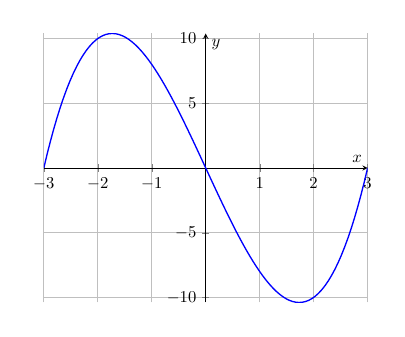
\begin{tikzpicture}[scale = 0.6]
    \begin{axis}[
        axis lines = middle,
        xlabel = $x$,
        ylabel = {$y$},
        domain=-3:3,
        samples=100,
        grid=both
    ]
    \addplot[blue, thick] {x^3 - 9 * x};
    \end{axis}
    \end{tikzpicture}
    \end{center}

    \begin{itemize}
        \item When $x < 0$, the curve is \textbf{Concave Down}
        \item When $x > 0$, the curve is \textbf{Concave Up}
    \end{itemize}

\end{example}

In the previous unit, we have discussed about the relationships between concavity and second derivative. 
\begin{proposition}
    [Concavity and Second Derivative] Give function $f(x)$, and its second derivative $f''(x)$. \\
    Let \(a,b\in\mathbb{R}\) with \(a<b\).
    $$I := (a, b) =  \{ x \in \R | a < x < b\}$$
    \[
        \forall x \in I, f''(x) > 0 \implies \text{\(f(x)\) is concave up on interval $I$}
    \]
    \[
        \forall x \in I, f''(x) < 0 \implies \text{\(f(x)\) is concave down on interval $I$}
    \]
\end{proposition}

There is also a relatinship between local maximum and minimum points. 
\begin{proposition}
    \begin{gather*}
    f:\mathbb{R}\to\mathbb{R} \\
    \forall a\in\mathbb{R},\quad \bigl(f'(a)=0 \land f''(a)<0\bigr)
    \implies f \text{ has a local maximum at } a \\
    \forall a\in\mathbb{R},\quad \bigl(f'(a)=0 \land f''(a)>0\bigr)
    \implies f \text{ has a local minimum at } a
    \end{gather*}
\end{proposition}

\begin{remark}
    A cusp can be considered a local maximum or minimum point but the test discussed in class may not be able to be applied. 

    $f'(a) = \text{ undefined }$ may also have $f''(a) = \text{ undefined}$
 \end{remark}

